%%MaD.tex - Notes taken for Materials and Devices Lecture
%%Author: Andy Goetz
%%Date Modified: 10-7-09
%%License: Ask me before reproducing/modifying, etc.


\documentclass{article}

%Make sure you have the file ShumanNote.scy in the same directory as
%this one. It has contains the style sheet for ECE111, and is needed
%to standardize the layout of LateX documents created for the class.
\usepackage{ShumanNotes} 
\usepackage{tikz}
\usepackage{program}
\usepackage{listings}
\lstset{
  showstringspaces=false
}
\pdfpagewidth 8.5in 
\pdfpageheight 11in

%This package is used to line up pictures 
\usepackage{graphicx}
\usepackage{fancyvrb}
\usepackage{listings}
%allows cursive font
%\usepackage{amsmath}

%allows hyperlinks 
\usepackage{hyperref}

\newcommand{\HRule}{\rule{\linewidth}{0.5mm}} 

\lhead{\leftmark}

\begin{document}



%% These commands allow me to use cursive letter for things such as
%% length.  Note that on ubuntu linux, this required installation of
%% the package 'texlive-fonts-extra'. 
%% Taken from
%% http://www.latex-community.org/forum/viewtopic.php?f=5&t=1404&start=0
\newenvironment{frcseries}{\fontfamily{frc}\selectfont}{}
\newcommand{\textfrc}[1]{{\frcseries#1}}
\newcommand{\mathfrc}[1]{\text{\textfrc{#1}}}

\setcounter{tocdepth}{2}

\begin{titlepage}
 
\begin{center}
 
 
\textsc{\LARGE ECE485/585 Microprocessor System Design}\\[1.5cm]
 
\textsc{\Large Portland State University}\\[0.5cm]
 
 
% Title
\HRule \\[0.4cm]
{ \huge \bfseries L1 Cache Simulation}\\[0.4cm]
 
\HRule \\[1.5cm]
 
% Author and supervisor
\begin{minipage}{0.4\textwidth}
\begin{center} \large
Andy \textsc{Goetz}, Bradon \textsc{Kanyid}, Eric \textsc{Krause}, and Kevin \textsc{Riedl}\\
\end{center}
\end{minipage}

 

 
 
\end{center}
\vfill
{ \textit{} }\\[4.0cm]
\begin{center}
% Bottom of the page
{\large \today}

\end{center} 
\end{titlepage}

\newpage

\textbf{\large Version}
\vspace{.1in}

\begin{tabular}{|p{1in}|p{4in}|p{1in}|}
\hline
\multicolumn{3}{|l|}{\textbf{Document Review}} \\ 
\hline
\textbf{Version}& \textbf{Comments} & \textbf{Date} \\ 
\hline
\textbf{1.0} & Initial release. & 12/3/2012 \\
\hline
\end{tabular}

\newpage


\section{Overview}

This project functionally simulates a split instruction/data L1 cache
for a 32-bit processor in a system with multiple processors.  The
system employs MESI protocol to ensure cache coherence.  The
instruction cache is 2-way set associative, consists of 16K sets, and
has 64-byte lines. The data cache is 4-way set associative, consists
of 16K sets, and has 64-byte lines.  Both caches employ LRU
replacement policy and are backed by an L2 cache (which is modeled as
a stub in this simulation).  Statistics regarding number of reads,
writes, hits, and misses are generated, as well as a hit percentage
rate.  This simulation has a single-cycle interface between a
processor and L1, and between L1 and L2.  All processor reads and
writes are a single byte.

\centerimage{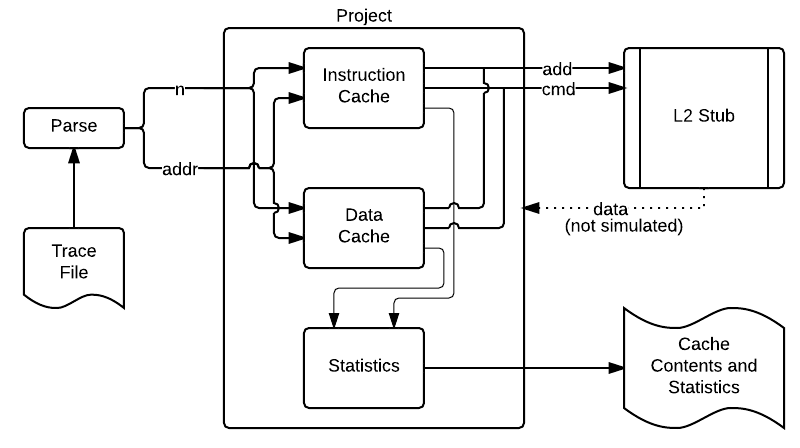
\includegraphics[width=5in]{585Final.png}}{Level 1 Diagram}{l1diag}

\newpage

\tableofcontents

\newpage

\section{Specification}




The 32-bit addresses from the processor are broken down into the
following fields:

\begin{center}
  \begin{tabular}{ll}
    \textbf{31:20} & = 12-bit tag \\
    \textbf{19:6} & = 14-bit index \\
    \textbf{5:0} & = 6-bit offset
  \end{tabular}
\end{center}

We specify the following method for interface with L2.  A 26-bit
address specifies a 64-byte cache line, and must be supplied with one
of the following 2-bit cmd\_out commands:

\begin{center}
  \begin{tabular}{ll}
    \textbf{00} & No Operation (ignore any input on address lines) \\
    \textbf{01} &  Read from L2\\
    \textbf{10} & Write to L2 \\
    \textbf{11} & Read with intent to modify
  \end{tabular}
\end{center}

In order to run, our simulation requires a trace file formatted using
the protocol specified in the project description.  A print command
will output human-readable cache contents and statistics.

\section{Assumptions}

In the course of designing our L1 cache, we were forced to make
several assumptions regarding the CPU it was designed for:

\begin{itemize}

\item \emph{The cache hierarchy is inclusive.} By making the L2
  cache support an inclusive policy, the synchronization logic
  between the L1 and L2 cache is greatly simplified.

\item \emph{The data cache is write-through.} The L1 and L2 caches
  together are required to support memory writebacks. However, because
  the cache design also needs to support MESI, we decided to implement
  the L1 data cache as a simple write-through cache. Because the cache
  hierarchy uses an inclusive policy, evictions forced by MESI in the
  L2 cache will force an eviction in the L1 cache. If the L1 cache had
  a dirty line, the MESI eviction would force a writeback to main
  memory in the L1, greatly complicating our code.

\item \emph{Cache contents (actual data) are irrelevant for this
  simulation.} Thus, all byte offsets are ignored.  Because we only
  stub out the processor, the next level cache, and our cache eviction
  policy is based entirely on memory addresses, there is no need to
  examine data values.

\item \emph{All read and write operations reference single byte
  locations.} In order to simplify the cache design, we assume that
  all reads and writes reference a single byte. This means we do not
  need to worry about supporting unaligned memory references.

\end{itemize}

\section{Pseudocode}

Pseudocode for the data and instruction caches are listed below:

\subsection{Data Cache}
\lstinputlisting{../pseudocode/datacache.txt}
\subsection{Instruction Cache}
\lstinputlisting{../pseudocode/inscache.txt}

\section{Testing}

In order to test our implementation, we developed a set of test
stimulus covering all of the corner cases. These tests are listed below. 

In addition to the testplan developed by our team, we also performed
blackbox testing with another ECE485 team. We traded testbenches, and
confirmed that both of our implementations produced the same hit
ratios.

\subsection{Cached\_Instr\_Reads.trace}
\begin{tabular}{|p{1.2in}|p{3.8in}|}
  \hline
  \textbf{Summary} & Multiple reads to the same instruction cache line.\\
  \hline
  \textbf{Expected Results} & Way 0 of Index 0 of Instruction Cache is valid. No
other ways are valid.\\
  \hline
  \textbf{Hit Ratio} & 75\%\\
  \hline
  \textbf{Test Vector} & \lstinputlisting{../vectors/Cached_Instr_Reads.trace} \\
  \hline
\end{tabular}


\subsection{Cached\_Data\_Reads.trace}
\begin{tabular}{|p{1.2in}|p{3.8in}|}
  \hline
  \textbf{Summary} & Multiple reads to the same data cache line.\\
  \hline
  \textbf{Expected Results} & Way 0 of Index 0 of Data Cache is valid. No other
ways are valid.\\
  \hline
  \textbf{Hit Ratio} & 75\%\\
  \hline
  \textbf{Test Vector} & \lstinputlisting{../vectors/Cached_Data_Reads.trace} \\
  \hline
\end{tabular}

\subsection{Interleaved\_Read\_Write.trace}
\begin{tabular}{|p{1.2in}|p{3.8in}|}
  \hline
  \textbf{Summary} & Reads and Writes to the data cache.\\
  \hline
  \textbf{Expected Results} & Way 0 of Index 0 of Data Cache is valid. No other
ways are valid.\\
  \hline
  \textbf{Hit Ratio} & 75\%\\
  \hline
  \textbf{Test Vector} & \lstinputlisting{../vectors/Interleaved_Read_Write.trace} \\
  \hline
\end{tabular}

\subsection{Same\_Set\_Instr.trace}
\begin{tabular}{|p{1.2in}|p{3.8in}|}
  \hline
  \textbf{Summary} & Multiple reads from the same set in the instruction cache.\\
  \hline
  \textbf{Expected Results} & Both ways of Index 0 are valid.\\
  \hline
  \textbf{Hit Ratio} & 0\%\\
  \hline
  \textbf{Test Vector} & \lstinputlisting{../vectors/Same_Set_Instr.trace} \\
  \hline
\end{tabular}

\subsection{Same\_Set\_Data.trace}
\begin{tabular}{|p{1.2in}|p{3.8in}|}
  \hline
  \textbf{Summary} & Multiple reads from the same set in the data cache. \\
  \hline
  \textbf{Expected Results} & All four ways of index 0 are valid.\\
  \hline
  \textbf{Hit Ratio} & 0\%\\
  \hline
  \textbf{Test Vector} & \lstinputlisting{../vectors/Same_Set_Data.trace} \\
  \hline
\end{tabular}

\subsection{Instr\_Conflict.trace}
\begin{tabular}{|p{1.2in}|p{3.8in}|}
  \hline
  \textbf{Summary} & Enough reads to the same instruction cache set to cause an eviction. \\
  \hline
  \textbf{Expected Results} & Both ways of index 0 are valid. LRU bit is 1. Way 0
                  has Tag 200 in it, Way 1 has 100 in it.\\
  \hline
  \textbf{Hit Ratio} & 0\%\\
  \hline
  \textbf{Test Vector} & \lstinputlisting{../vectors/Instr_Conflict.trace} \\
  \hline
\end{tabular}

\subsection{Data\_Conflict.trace}
\begin{tabular}{|p{1.2in}|p{3.8in}|}
  \hline
  \textbf{Summary} & Enough reads and writes to the same instruction cache set to
         cause an eviction.\\
  \hline
  \textbf{Expected Results} & All ways of index 0 are valid. LRU way is 1. Way 0
                  has 500 in it, Wa 1 has 200 in it, way 2 has 300 in
                  it, and way 3 has 400 in it.\\
  \hline
  \textbf{Hit Ratio} & 0\%\\
  \hline
  \textbf{Test Vector} & \lstinputlisting{../vectors/Data_Conflict.trace} \\
  \hline
\end{tabular}

\subsection{Instr\_Invalidate.trace}
\begin{tabular}{|p{1.2in}|p{3.8in}|}
  \hline
  \textbf{Summary} & Multiple Reads Followed by Invalidate clears single line. \\
  \hline
  \textbf{Expected Results} & way 0 of index 0 is invalid, way 1 of index 0 is
                  valid.\\
  \hline
  \textbf{Hit Ratio} & 0\%\\
  \hline
  \textbf{Test Vector} & \lstinputlisting{../vectors/Instr_Invalidate.trace} \\
  \hline
\end{tabular}

\subsection{Data\_Invalidate.trace}
\begin{tabular}{|p{1.2in}|p{3.8in}|}
  \hline
  \textbf{Summary} & Multiple Reads Followed by Invalidate clears single line.\\
  \hline
  \textbf{Expected Results} & way 1 of index 0 of data cache invalid, rest of ways of index 0 valid.\\
  \hline
  \textbf{Hit Ratio} & 0\%\\
  \hline
  \textbf{Test Vector} & \lstinputlisting{../vectors/Data_Invalidate.trace} \\
  \hline
\end{tabular}

\subsection{Instr\_Clear.trace}
\begin{tabular}{|p{1.2in}|p{3.8in}|}
  \hline
  \textbf{Summary} & Read Followed by Clear empties data cache.\\
  \hline
  \textbf{Expected Results} & No ways in instruction cache are valid.\\
  \hline
  \textbf{Hit Ratio} & 0\%\\
  \hline
  \textbf{Test Vector} & \lstinputlisting{../vectors/Instr_Clear.trace} \\
  \hline
\end{tabular}

\subsection{Data\_Clear.trace}
\begin{tabular}{|p{1.2in}|p{3.8in}|}
  \hline
  \textbf{Summary} & Read followed by Clear empties data cache.\\
  \hline
  \textbf{Expected Results} & All ways of Data Cache are invalid.\\
  \hline
  \textbf{Hit Ratio} & 0\%\\
  \hline
  \textbf{Test Vector} & \lstinputlisting{../vectors/Data_Clear.trace} \\
  \hline
\end{tabular}

\subsection{Instr\_Invalidate\_read.trace}
\begin{tabular}{|p{1.2in}|p{3.8in}|}
  \hline
  \textbf{Summary} & Read, Invalidate, Read uses cleared way as LRU.\\
  \hline
  \textbf{Expected Results} & Way 0 of index 400 has tag of 001. Way 1 of index
                  400 has tag of 003.\\
  \hline
  \textbf{Hit Ratio} & 0\%\\
  \hline
  \textbf{Test Vector} & \lstinputlisting{../vectors/Instr_Invalidate_read.trace} \\
  \hline
\end{tabular}

\subsection{Data\_Invalidate\_read.trace}
\begin{tabular}{|p{1.2in}|p{3.8in}|}
  \hline
  \textbf{Summary} & Read, Invalidate, Read uses cleared way as LRU.\\
  \hline
  \textbf{Expected Results} & Index 400 of data cache has tag 001 in way 0, tag
                  002 in way 1, tag 005 in way 2, and tag 004 in way 3.\\
  \hline
  \textbf{Hit Ratio} & 0\%\\
  \hline
  \textbf{Test Vector} & \lstinputlisting{../vectors/Data_Invalidate_read.trace} \\
  \hline
\end{tabular}

\newpage

\section {Source Code}

The Verilog source code for our project is reproduced below:

\subsection{memtest.v}
\lstinputlisting[language=Verilog]{../BEEFA55/Source/memtest.v}
\newpage 

\subsection{PROJECT.v}
\lstinputlisting[language=Verilog]{../BEEFA55/Source/PROJECT.v}
\newpage 

\subsection{INS\_CACHE.v}
\lstinputlisting[language=Verilog]{../BEEFA55/Source/INS_CACHE.v}
\newpage 

\subsection{DATA\_CACHE.v}
\lstinputlisting[language=Verilog]{../BEEFA55/Source/DATA_CACHE.v}
\newpage 

\subsection{STATS.v}
\lstinputlisting[language=Verilog]{../BEEFA55/Source/STATS.v}
\newpage 

\section{Testbench Output}

The output of our tests is reproduced below. 

\lstinputlisting{../vectors/testresults}
\end{document}
